\section{Information theory}
\label{sec:infoth}
How to quantify information and discrepancies between probability distributions is at the heart of machine learning and an important prerequisite for understanding our contributions of \Cref{chapter:icf}, \Cref{chapter:smcp} and \Cref{chapter:hfc}.

\subsection{Probability distribution and density/mass function}
For simplicity, in this section, we will not introduce the notion of probability distribution in its most general form using measure theory, but only using probability density functions. For a more complete treatment, please refer to~\citet{kolmogorov2018foundations, billingsley2008probability}.

\begin{definition}[Probability Mass Function (pmf)]
Let us consider a discrete random variable $X \in \gX$ where $\gX$ is discrete and a function $p: \gX \mapsto \R$. We say that $p$ is the probability mass function of $X$ if
\begin{enumerate}
    \item $p(x) \ge 0, \forall x \in \gX$
    \item $\sum_{x \in \gX} p(x) = 1$
    \item $\mathbb{P}(X = x) = p(x)$
\end{enumerate}
\end{definition}

In the context of continuous random variables, we can define the notion of \emph{probability density function} which has a very similar definition.
\begin{definition}[Probability Density Function (pdf)]
Let us consider a random variable $X \in \gX$ and a function $p: \gX \mapsto \R$. We say that $p$ is the probability density function of $X$ if
\begin{enumerate}
    \item $p(x) \ge 0, \forall x \in \gX$
    \item $\int_\gX p(x) dx = 1$
    \item $\mathbb{P}(a \le X \le b) = \int_a^b p(x) dx$
\end{enumerate}
\end{definition}

We will make use of this concept extensively as most machine learning methods can be understood as trying to approximate a distribution $p$ (for instance the data distribution) with an approximate distribution $q$.



\subsection{Divergences}
While distances are the typical notion used for comparing mathematical objects, a weaker notion, called divergences are often used to compare probability measures.



\begin{definition}[Distance]
A function $d$ on a set $\gX$ between two objects $x$ and $y \in \gX$ must satisfy four properties to be a distance
\begin{enumerate}
    \item \emph{non-negativity:} $d(x, y) \ge 0$
    \item \emph{identity of indiscernibles:} $d(x,y) = 0$ if and only if $x = y$
    \item \emph{symmetry:} $d(x,y) = d(y,x)$
    \item \emph{triangle inequality:} $\forall z \in \gX, \ d(x, y) \le d(x,z) + d(z, y) $
\end{enumerate}
\end{definition}

A divergence, on the other hand, only requires the \emph{non-negativity} and \emph{identity of the indiscernibles} properties and is defined for probability distributions.

\begin{definition}[Divergence]
A function $\gD(\cdot || \cdot)$ between two distributions $p$ and $q$ must satisfy two properties to be a divergence
\begin{enumerate}
    \item \emph{non-negativity:} $\gD(p||q) \ge 0$
    \item\emph{identity of indiscernibles:} $\gD(p||q) = 0$ if and only if $p = q$
\end{enumerate}
\end{definition}


The most emblematic divergence, especially in machine learning and generally Maximum Likelihood Estimation (MLE) is certainly the Kullback-Leibler divergence~\citep{kullback1951information, kullback1997information}.
\begin{example}[Kullback-Leibler divergence] The Kullback-Leibler divergence is defined by
\begin{equation}
\label{eq:kl}
    \KL(p||q) = \int_{x \in \gX} p(x) \log \frac{p(x)}{q(x)}  dx
\end{equation}
\end{example}

The Kullback-Leibler divergence contains the term $-\int_{x \in \gX}  p(x) \log q(x) dx$ which is the negative log-likelihood of $q$ under the distribution $p$, which is also known as the \emph{cross-entropy}. This divergence is very common in machine learning as we will see in \Cref{sec:ml}.

\subsection{Measures of information}
Now that we have defined the fundamental notions of probabilities and divergences, we can make us of them to build useful concepts from information theory such as \emph{entropy} or \emph{mutual information}.


The notion of entropy is fundamental in physics where it was first introduced by Boltzmann. \citet{shannon1948mathematical} transcribed the concept to communication theory and it is now used widely in statistics and machine learning. For a discrete random variable $X$ with mass function $p$, the entropy $H(X)$ of $X$ is  

\begin{equation}
\label{eq:entropy}
    H(X) = - \sum_{x \in \gX} p(x) \log p(x)
\end{equation}

Entropy should be understood as the \emph{information} necessary to describe $p$. As such, the entropy is always positive $H(X) \ge 0$, it is equal to $0$ only when $p$ is a Dirac function, in that case $p$ does not contain any uncertainty.
$H(X)$ is also bounded by number of values $X$ can take: $H(X) \le \log | \gX |$ which is achieved when $p$ is the uniform distribution, the distribution with maximal uncertainty. Note that entropy can be defined in the same way for continuous variables, we call this the \emph{differential entropy} $h(X) = - \int_{\gX} p(x) \log (x) dx$ but we lose the upper and lower bounds described above.

Using the notion of Kullback-Leibler divergence notion defined above and by defining the uniform distribution whose probability mass function is $u(x) = \frac{1}{|\gX|}, \ \forall x \in \gX$, we have

\begin{eqnarray*}
    \KL(p||u) &=& \sum_{x \in \gX} p(x) \log \frac{p(x)}{u(x)} 
    =\log |\gX| - H(X)
\end{eqnarray*}
Thus, entropy can also be interpreted as a measure of how close we are to the uniform distribution.

If we consider the case where we have two random variables $X$ and $Y$ with joint probability mass function $p(x, y)$ and marginals $p(x)$ and $p(y)$ we can write the joint entropy as
\begin{eqnarray*}
H(X,Y) &=& - \sum_{x, y} p(x,y) \log p(x,y)\\ 
 &=& - \sum_{x, y} p(x,y) \big(\log p(y|x) - \log p(x) \big)\\ 
  &=& - \sum_x p(x) \sum_{y} p(y|x) \log p(y|x) - \sum_x p(x) \log p(x)\\ 
  &=& H(Y|X) + H(X)
\end{eqnarray*}
 where we defined $H(Y|X) = - \sum_x p(x) \sum_{y} p(y|x) \log p(y|x)$, the \emph{conditional entropy}. $H(Y|X)$ should be understood as the amount of information necessary to describe $Y$ given that we know everything about $X$.

Finally we can introduce the idea of \emph{mutual information}, \textit{i.e} how much information is shared between $X$ and $Y$.
The mutual information $\gI(X, Y)$ can be written in several different manners

\begin{eqnarray*}
    \gI(X, Y) &=& H(X) + H(Y) - H(X, Y)\\
    &=& H(X) - H(X|Y)\\
    &=& \sum_{x, y} p(x,y) \log \frac{p(x,y)}{p(x) p(y)}\\
    &=& \KL\big(p(x,y)||p(x) p(y)\big)
\end{eqnarray*}
see Figure~\ref{fig:mutual_info} for a schematic view.

Another useful interpretation of mutual information is to see it as the divergence between the joint probability and the product of the marginals. When $X$ and $Y$ and conditional independent, the divergence, thus mutual information, is $0$. The concept of mutual information is especially relevant in reinforcement learning where it has been used (in many different ways) as an intrinsic reward signal~\citep{still2012information, mohamed2015variational, gregor2016variational, thomas2018disentangling, eysenbach2018diversity, eslami2018neural}.



\begin{figure}
\centering


\tikzset{every picture/.style={line width=0.75pt}} %

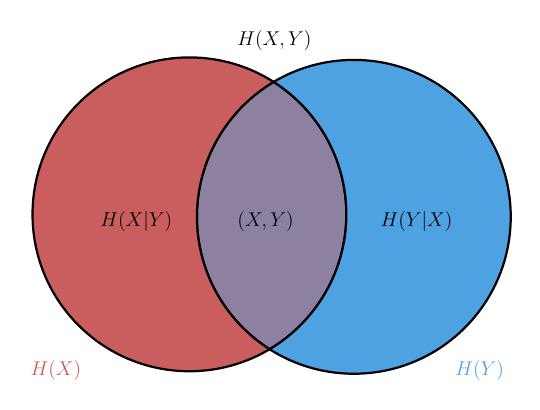
\begin{tikzpicture}[thick,scale=0.6, every node/.style={transform shape}, x=0.75pt,y=0.75pt,yscale=1,xscale=1]

\draw  [fill={rgb, 255:red, 141; green, 128; blue, 160 }  ,fill opacity=1 ] (389,241) .. controls (389,285.7) and (365.72,324.97) .. (330.62,347.34) .. controls (293.72,325.36) and (269,285.07) .. (269,239) .. controls (269,194.3) and (292.28,155.03) .. (327.38,132.66) .. controls (364.28,154.64) and (389,194.93) .. (389,241) -- cycle ;
\draw  [fill={rgb, 255:red, 202; green, 93; blue, 93 }  ,fill opacity=1 ] (263,115) .. controls (286.52,115) and (308.54,121.44) .. (327.38,132.66) .. controls (292.28,155.03) and (269,194.3) .. (269,239) .. controls (269,285.07) and (293.72,325.36) .. (330.62,347.34) .. controls (311.08,359.79) and (287.88,367) .. (263,367) .. controls (193.41,367) and (137,310.59) .. (137,241) .. controls (137,171.41) and (193.41,115) .. (263,115) -- cycle ;
\draw  [fill={rgb, 255:red, 79; green, 162; blue, 226 }  ,fill opacity=1 ] (395,365) .. controls (371.48,365) and (349.46,358.56) .. (330.62,347.34) .. controls (365.72,324.97) and (389,285.7) .. (389,241) .. controls (389,194.93) and (364.28,154.64) .. (327.38,132.66) .. controls (346.92,120.21) and (370.12,113) .. (395,113) .. controls (464.59,113) and (521,169.41) .. (521,239) .. controls (521,308.59) and (464.59,365) .. (395,365) -- cycle ;

\draw (300,390) node [anchor=north west][inner sep=0.75pt]   [align=left] {\large $ H(X, Y) $};
\draw (415,245) node [anchor=north west][inner sep=0.75pt]   [align=left] {\large $ H(Y|X) $};
\draw (300,245) node [anchor=north west][inner sep=0.75pt]   [align=left] {\large $\gI(X, Y) $};
\draw (134,125) node [anchor=north west][inner sep=0.75pt]   [align=left] {\textcolor[rgb]{0.79,0.36,0.36}{\large $ H(X) $}};
\draw (475,125) node [anchor=north west][inner sep=0.75pt]   [align=left] {\textcolor[rgb]{0.31,0.64,0.89}{\large $ H(Y) $}};
\draw (190,245) node [anchor=north west][inner sep=0.75pt]   [align=left] {\large $ H(X|Y) $};


\end{tikzpicture}


    \caption{Mutual information is the information shared between $X$ and $Y$. From this Venn diagram, we recover the first two definitions of the mutual information in term of the joint and conditional entropy. For instance the red circle represents the entropy associated to $X$, but as the purple intersection is the mutual information between $X$ and $Y$, the red circle minus the purple intersection represents the uncertainy of $X$ conditioned on us knowing $Y$, i.e $H(X|Y)$.}
    \label{fig:mutual_info}
\end{figure}

























